\documentclass{article}
\usepackage[a4paper, tmargin=1in, bmargin=1in]{geometry}
\usepackage[utf8]{inputenc}
\usepackage{graphicx}
\usepackage{parskip}
\usepackage{pdflscape}
\usepackage{listings}
% \usepackage{float}
%\usepackage{hyperref}
%\usepackage{titlesec}

\newcommand{\ra}{$\rightarrow$}


% \title{\vspace{-4.0cm} EE 344 Project Proposal \\ Visible Light Communication using LED}
% \author{
%   Group No. B-05\\
%   Faculty Incharge: Prof. Kumar Appaiah\\
%   Arka Sadhu - 140070011\\
%   Sudeep Salgia - 14D070011\\
%   Parth Kothari - 14D070019\\
% }

% \date{\today}

\begin{document}
% \maketitle

EE 344 Project Report 1 : Visible Light Communication using LED\\
Group No. B-05\\
Faculty Incharge: Prof. Kumar Appaiah\\
% Group Members:\\
Arka Sadhu - 140070011\\
Sudeep Salgia - 14D070011\\
Parth Kothari - 14D070019\\
% \hline
\vspace{-1.0cm}

\section{Work Promised}

\begin{itemize}
\item Finish Tackling the Problem of Clock Synchronization and Frequency offset
\item Start integrating the components.
\item Code the modulation the demodulation schemes in the microcontroller
% \item Procurement of components : The SD card reader is yet to arrive. We have placed an order for the same.
% \item Finishing the transmitter ciruit
% \item Getting started with the receiver circuit
\end{itemize}

\section{Work Accomplished }
% Five to ten sentences providing a non-technical description; use technical words only to describe important specifications. Describe the “big picture” of the project.

\subsection{Block Diagram and Demonstration}
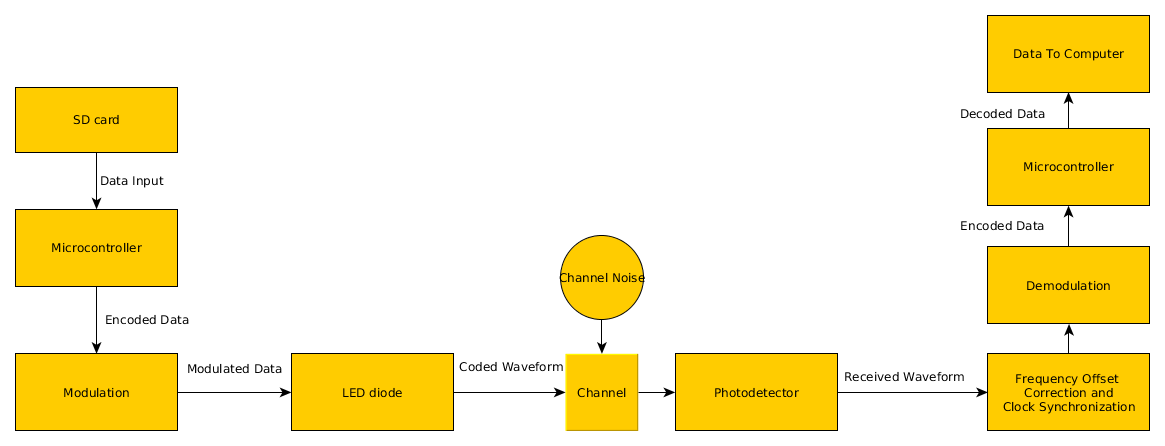
\includegraphics[scale=0.3]{functional_flow}
\\%What we will show
\subsection{Software Implementation}
\begin{itemize}
\item Implemented Transmitter code with (On-Off Keying) OOK with the encoding scheme : $'0' \Rightarrow '01'$ and $'1' \Rightarrow '10'$
\item Also implemented Transmission using an USB interface.
\item Implemented Receiver code with the decode scheme : $'01' \Rightarrow '0'$ and $'10' \Rightarrow '1'$
\end{itemize}

\subsection{Hardware Implementation}
\begin{itemize}
\item Added better features to the receiver circuit like comparator and noise filter(to filter out static AC of 50Hz)
\item The clock is getting synchronized in the Phase Locked Loop (PLL) circuit.
\item Integrated the transmitter, receiver and the PLL circuit, with clock synchronization, currently working with 40kHz.
  % \item In short, whole hardware is working at 40kHz
\end{itemize}

\section{Testing}

We tested each of the components in a sequential manner in order to ensure the integrity of each component.
\begin{itemize}
\item Given a sequence of 1's and 0's of frequency 40kHz, and the PLL locks successfully at 40kHz.
\item Both the Transmitter and Receiver codes were debugged using Hardware breakpoints, and testing the same on the DSO.
\end{itemize}

\section{Problems Faced}

\begin{itemize}
\item Constructing the differentiator of Alexander Hogge Phase Detector circuit was difficult to think about, but later we implented with combination of NOT and AND gates.
\item As the frequency increased the waveform of the receiver became more and more distorted (was occuring during Eval-1) at high frequencies. We overcame this using a comparator.
\item During the implementation and testing of the code DSO was not available, and since there is no Logic Analyzer in Code Composer Studio, it was not possible to check the actual waveforms.
\item When the USB is connected it sends some 29 random values, and we are finding it difficult to weed these random values out and this bug is yet to be solved.
\end{itemize}


\section{Goals for the next evaluation}

\begin{itemize}
\item Increase the data rate as high as possible.
\item Make the whole circuit on a PCB and package it.
\item Integrate the Software and Hardware.
  % \item Code the modulation the demodulation schemes in the microcontroller
\end{itemize}

\end{document}

